 Due to the fast evolution of the LHC machine, with a rapid rise in the
instantaneous luminosity, the data taking conditions have changed
rapidly.  In particular it is difficult to exactly reproduce the
number of overlapping events (i.e. pile-up) between data and
simulation, and thus there will be differences in the number of
reconstructed primary vertices. We correct this disagreement by
reweighting the simulation to match the number of pileup events in data. 

The target pileup distribution for data is generated using the instantaneous luminosity 
per bunch crossing for each luminosity section, stored in the LumiDB database, 
and the total pp inelastic cross section of $68$mb, integrated over the 
full data-taking period. A poissonian smearing is applied to model
statistical fluctuations in the actual number of pileup events 
present in the data. The source distribution is taken from the PileupInfo
collection which stores the true number of pileup events mixed with the 
particular hard interaction process in each Monte Carlo event. Comparisons of the
pileup distribution from the Summer11 Monte Carlo samples and the pileup 
distribution from various periods of data-taking is shown in Figure 
\ref{fig:NPU}. The resulting weighting factors are shown in Figure 
\ref{fig:PUReweightingFactors}. 

 
\begin{figure}[hbt]
\begin{center}
%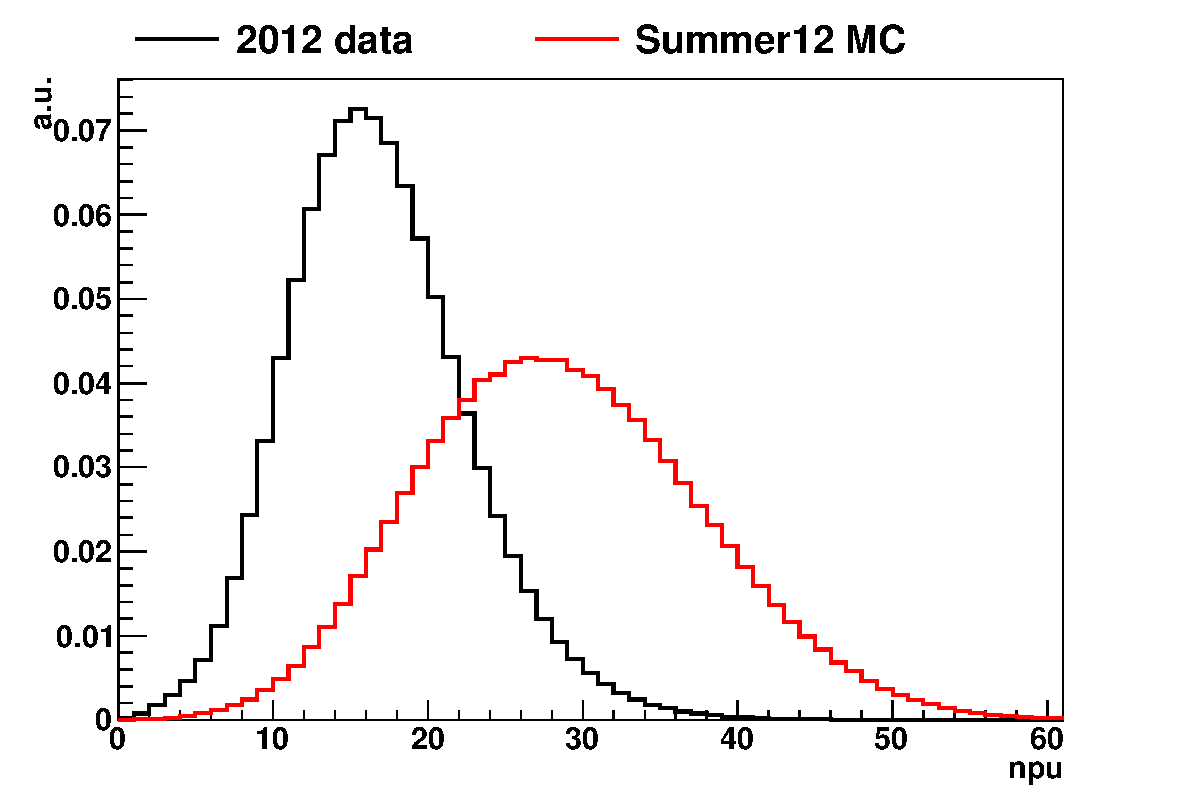
\includegraphics[width=0.7\linewidth]{figures/NPUDistributions.pdf}
\caption{\label{fig:NPU} Comparison of the number of pileup interactions 
for the Monte Carlo and various periods of 2011 data.}
\end{center}
\end{figure}

\begin{figure}[hbt]
\begin{center}
%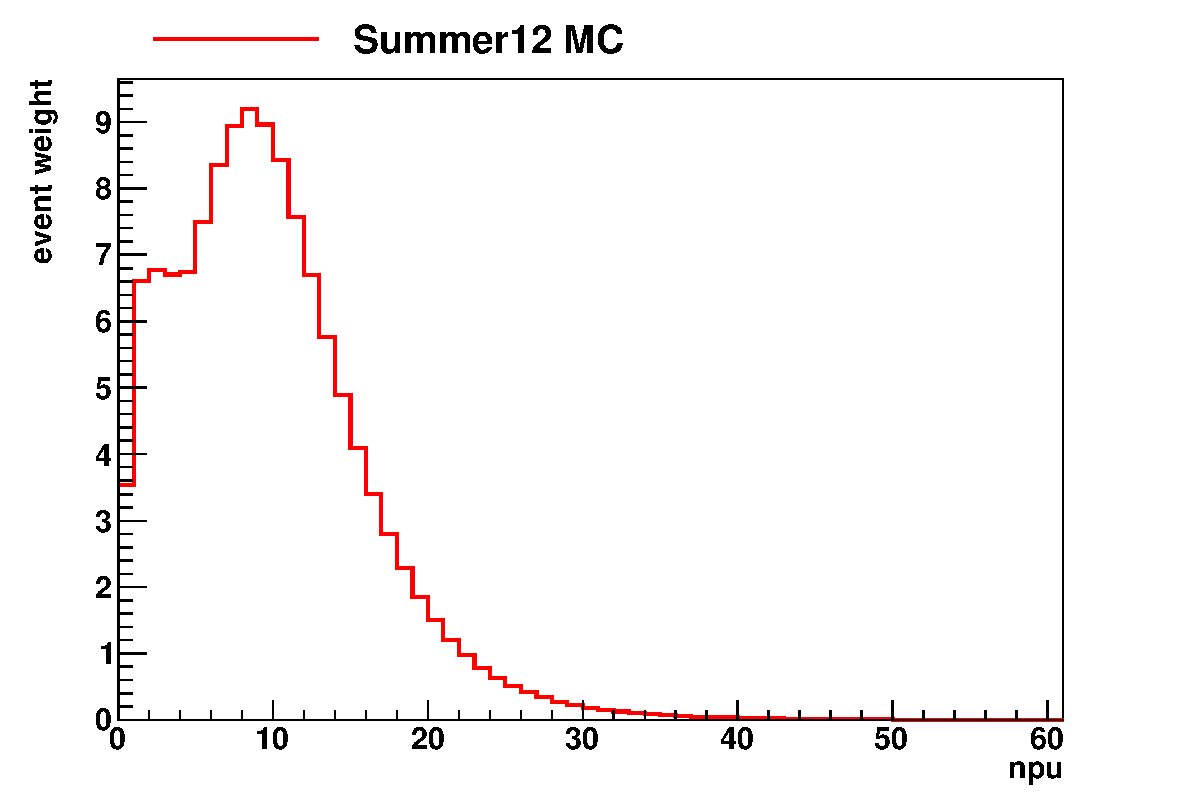
\includegraphics[width=0.7\linewidth]{figures/ReweightingFactors.pdf}
\caption{\label{fig:PUReweightingFactors} Pileup reweighting factors for various periods of 2011 data.}
\end{center}
\end{figure}


A cross check of this procedure is performed by comparing the number of 
reconstructed primary vertices and the event energy density ($\rho$)
from \zmm\ events in data and Monte Carlo. The comparisons are shown in
Figures \ref{fig:PUValidation_Run2011A},\ref{fig:PUValidation_Run2011B},
and \ref{fig:PUValidation_Full2011} for Run2011A, Run2011B, and the 
total 2011 combined data, respectively. The residual differences 
reflect the size of the systematic uncertainty in the determination 
of the amount of pileup present in the data. Since the dependence 
of the efficiencies for selecting signal and background events on 
pileup are small, this systematic uncertainty due to the pileup 
is small when propagated to the final 
result.

\begin{figure}[hbt]
\begin{center}
%\subfigure[Number of reconstructed vertices]{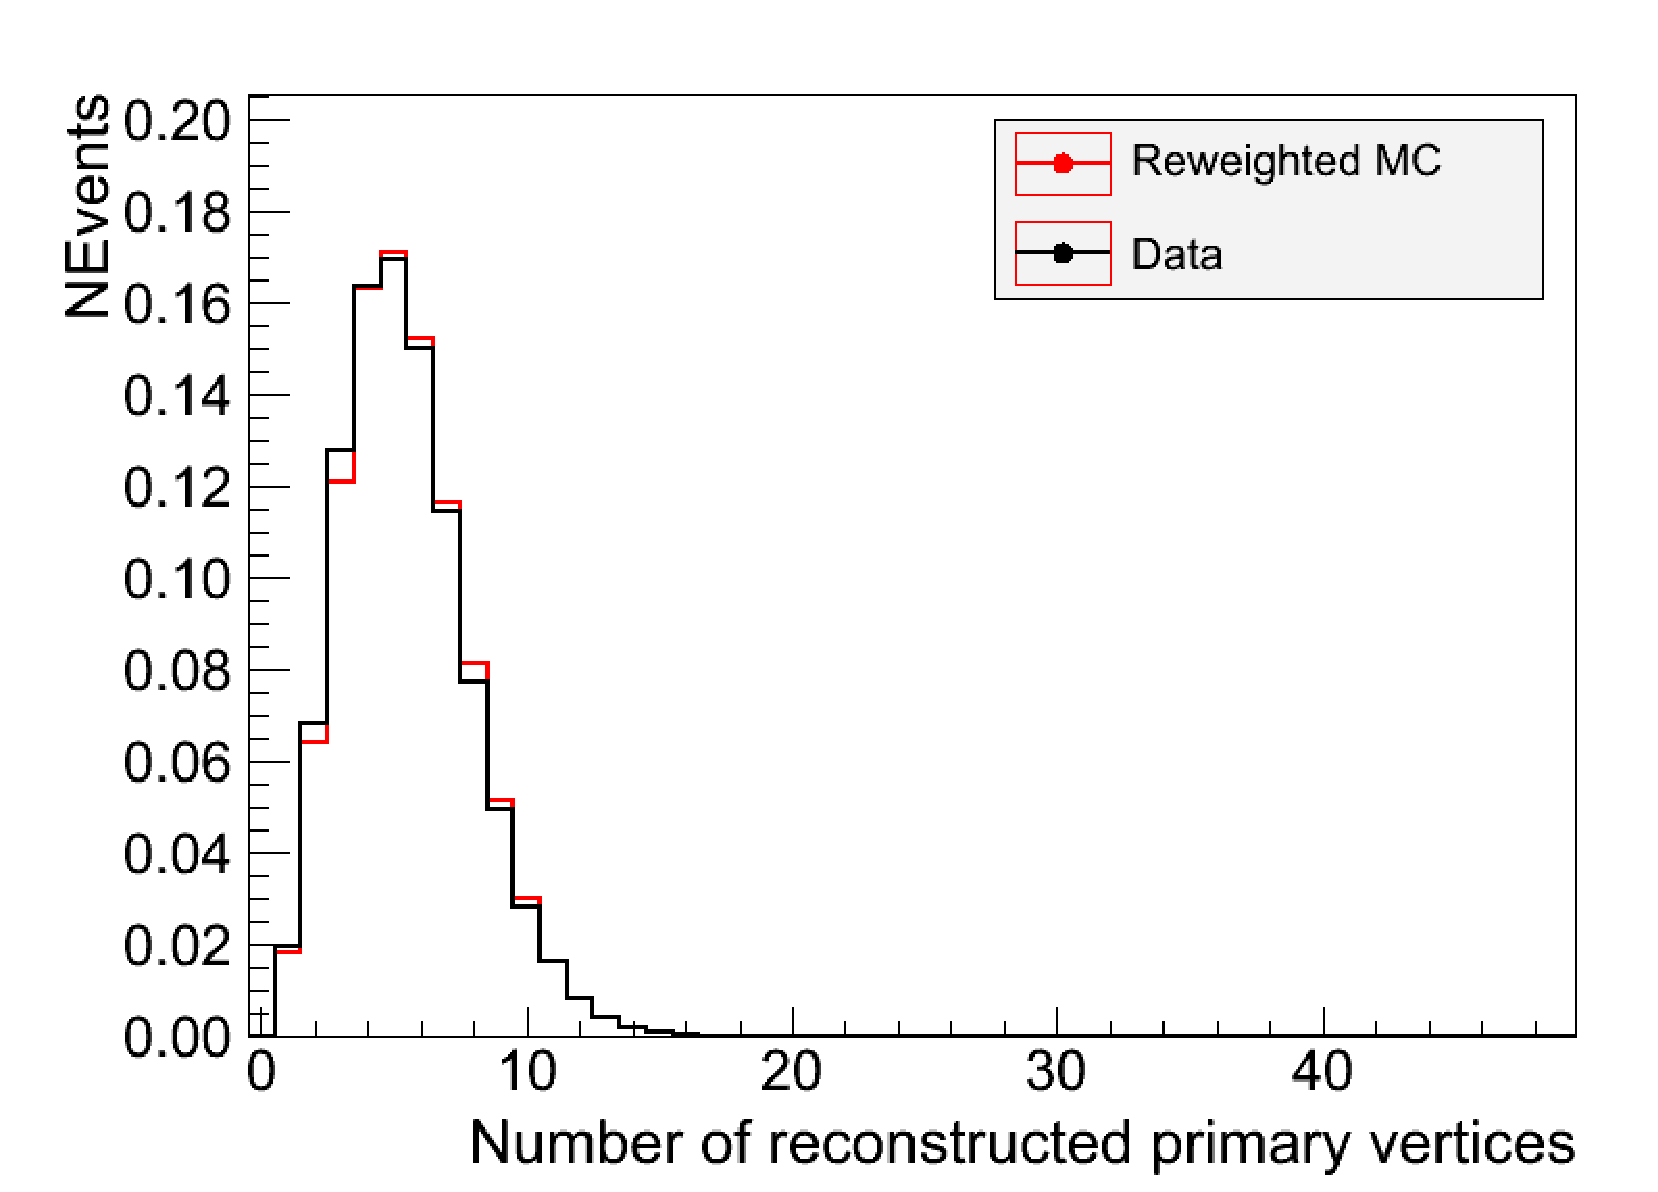
\includegraphics[width=0.45\linewidth]{figures/PileupReweightingValidation_NVtx_SmurfV6DYmm_Run2011A.pdf}}
%\subfigure[Event energy density ($\rho$)]{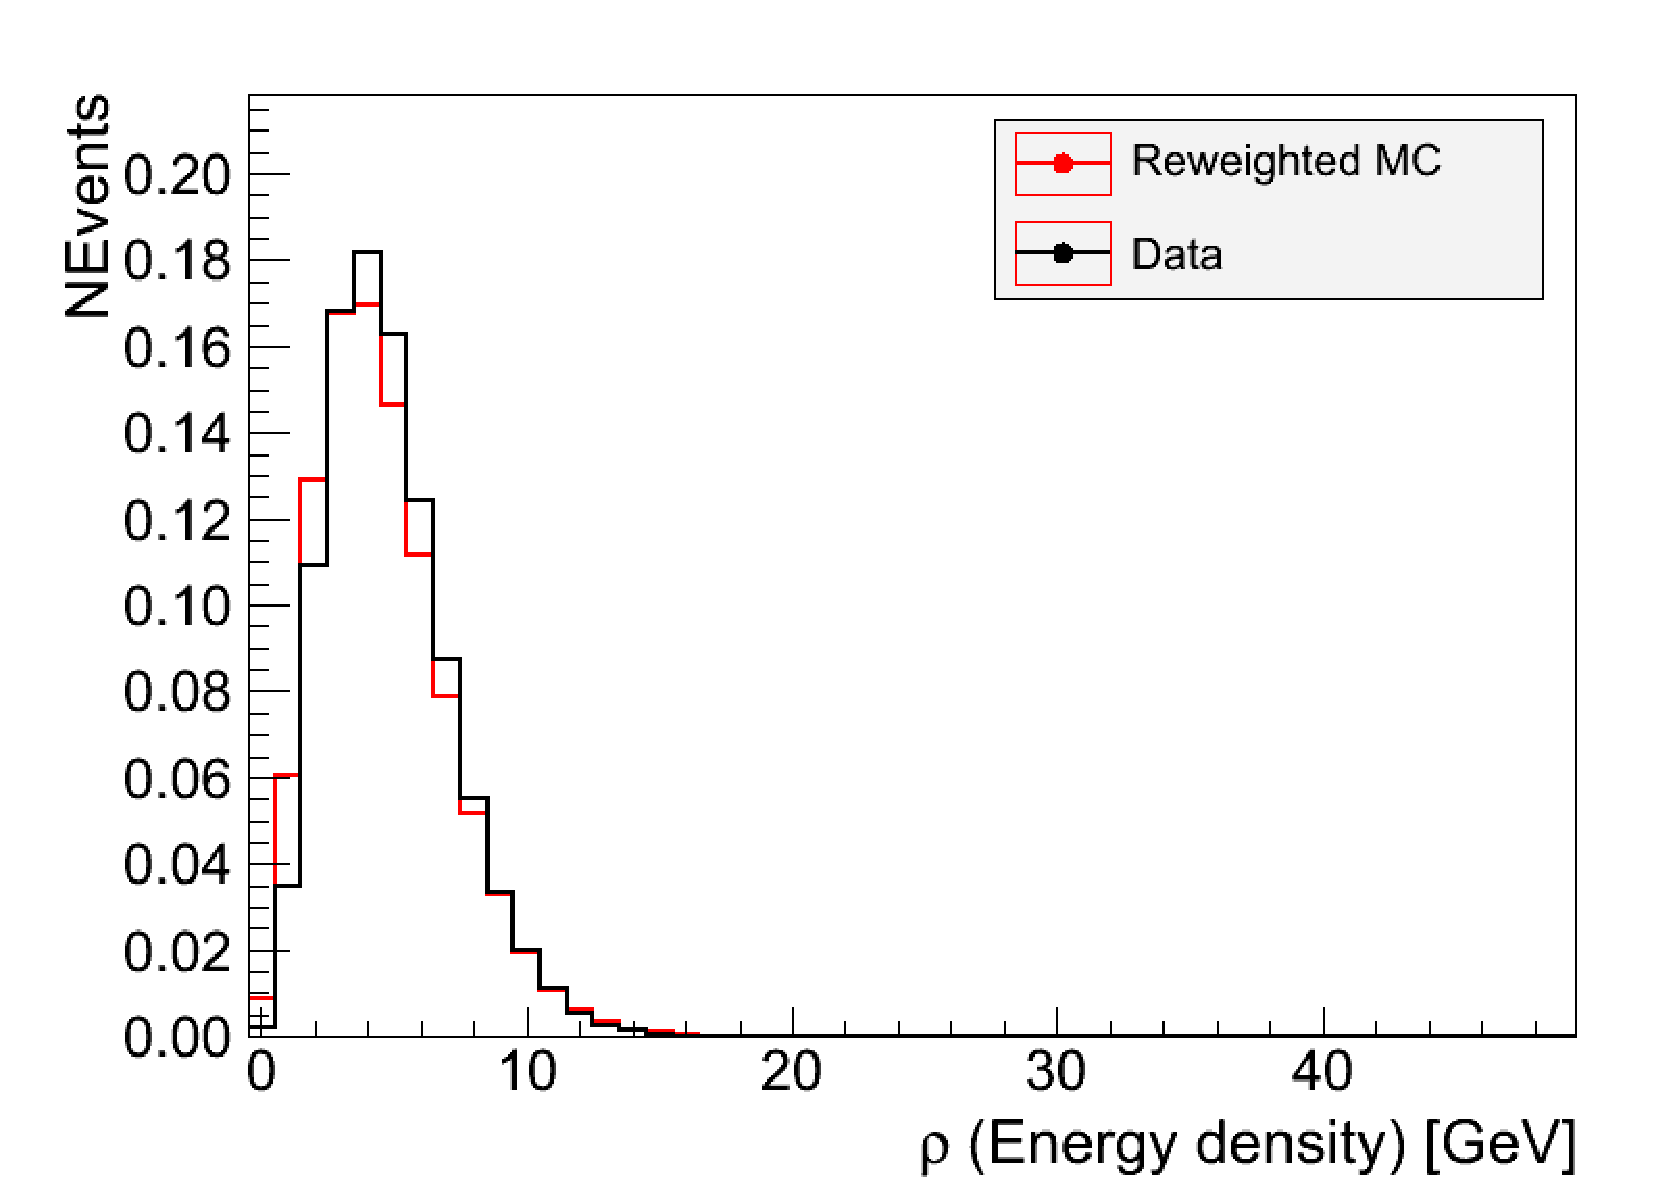
\includegraphics[width=0.45\linewidth]{figures/PileupReweightingValidation_Rho_SmurfV6DYmm_Run2011A.pdf}}
\caption{\label{fig:PUValidation_Run2011A} Number of reconstructed primary vertices (a) and
the event energy density (b) for data and Monte Carlo reweighted in the number
of pileup events for the Run2011A dataset.}
\end{center}
\end{figure}

\begin{figure}[hbt]
\begin{center}
%\subfigure[Number of reconstructed vertices]{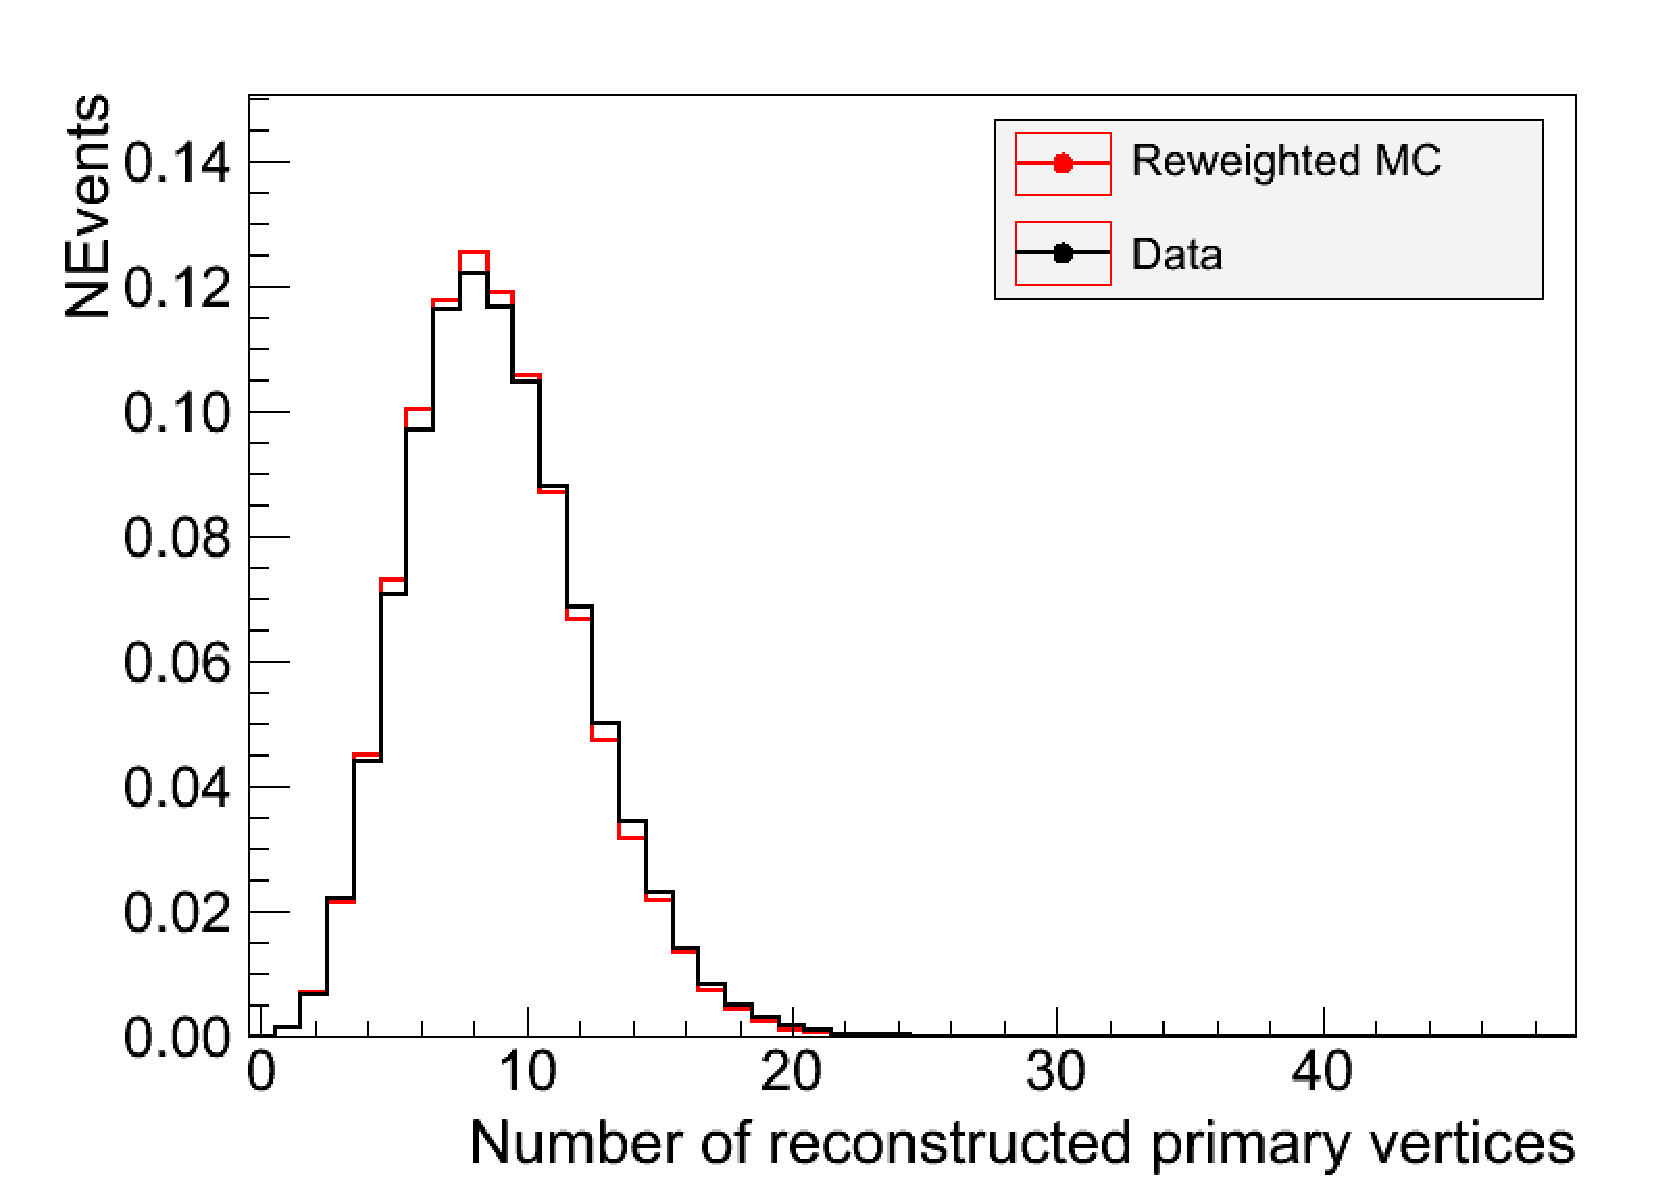
\includegraphics[width=0.45\linewidth]{figures/PileupReweightingValidation_NVtx_SmurfV6DYmm_Run2011B.pdf}}
%\subfigure[Event energy density ($\rho$)]{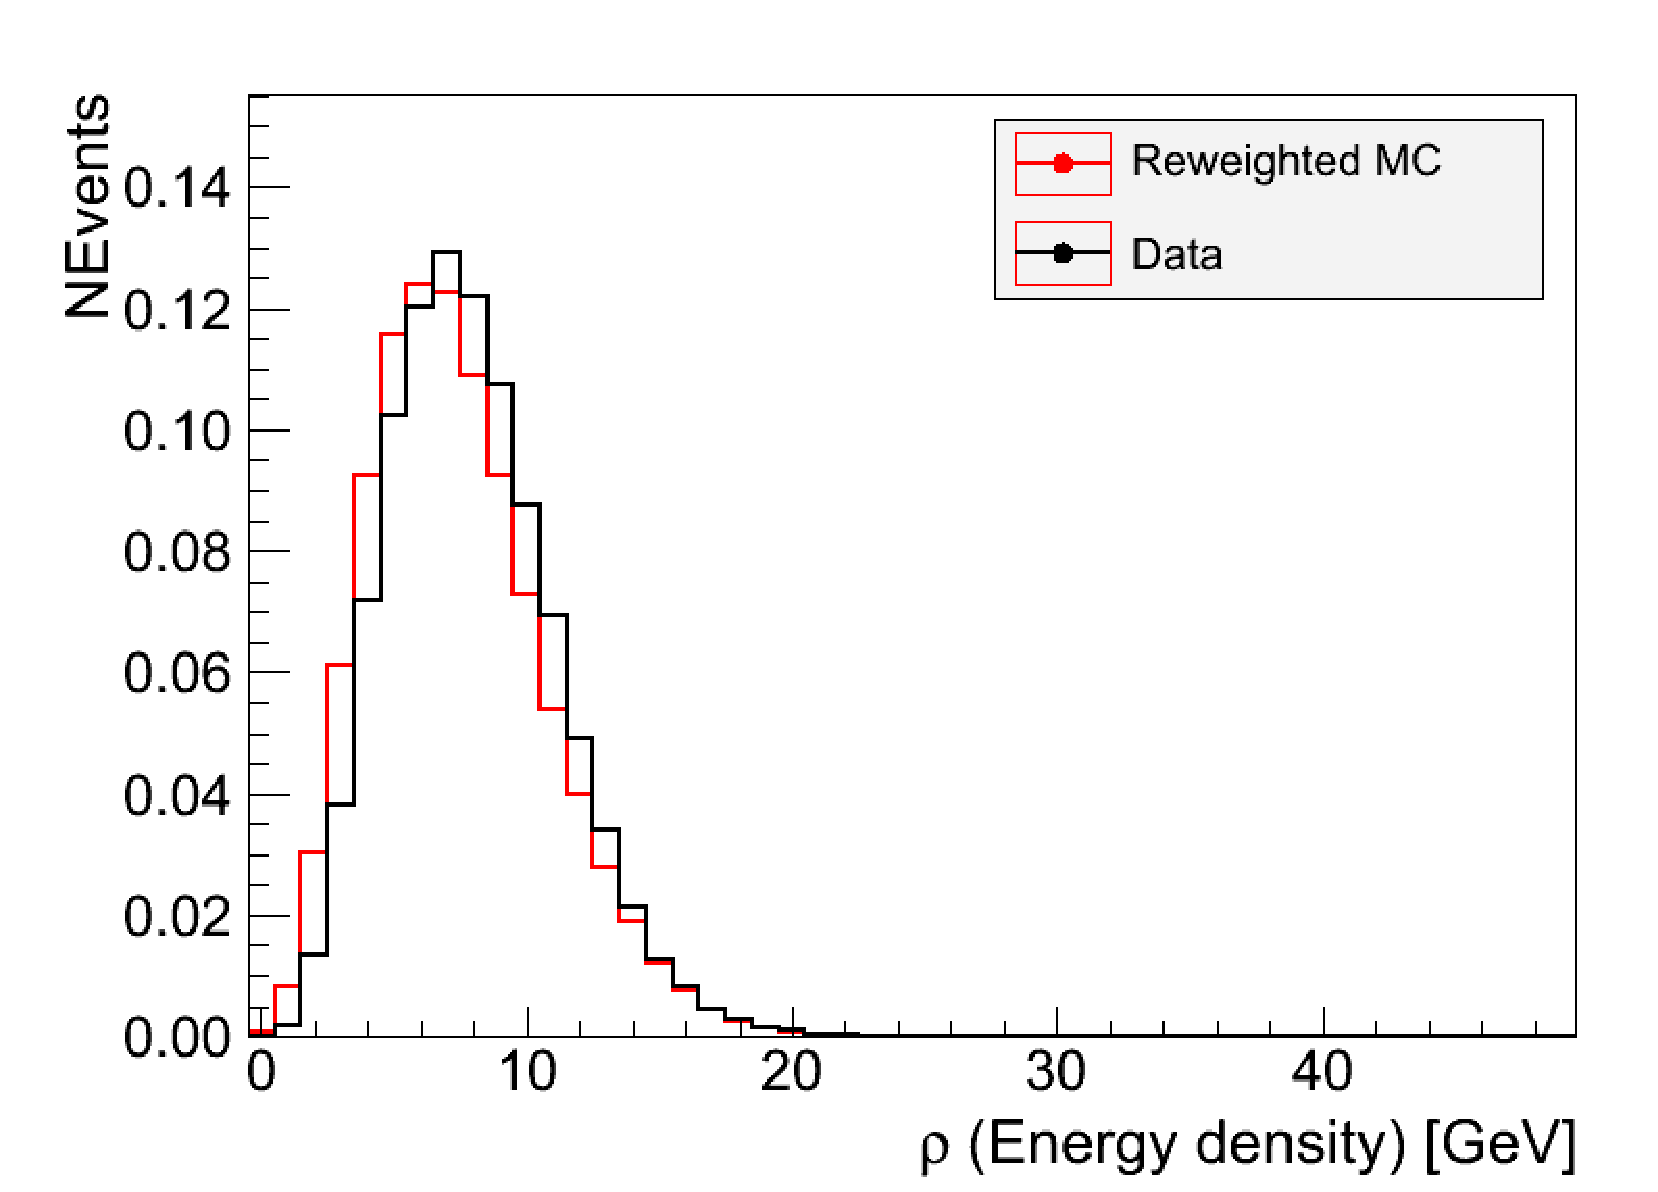
\includegraphics[width=0.45\linewidth]{figures/PileupReweightingValidation_Rho_SmurfV6DYmm_Run2011B.pdf}}
\caption{\label{fig:PUValidation_Run2011B} Number of reconstructed primary vertices (a) and
the event energy density (b) for data and Monte Carlo reweighted in the number
of pileup events for the Run2011B dataset.}
\end{center}
\end{figure}

\begin{figure}[hbt]
\begin{center}
%\subfigure[Number of reconstructed vertices]{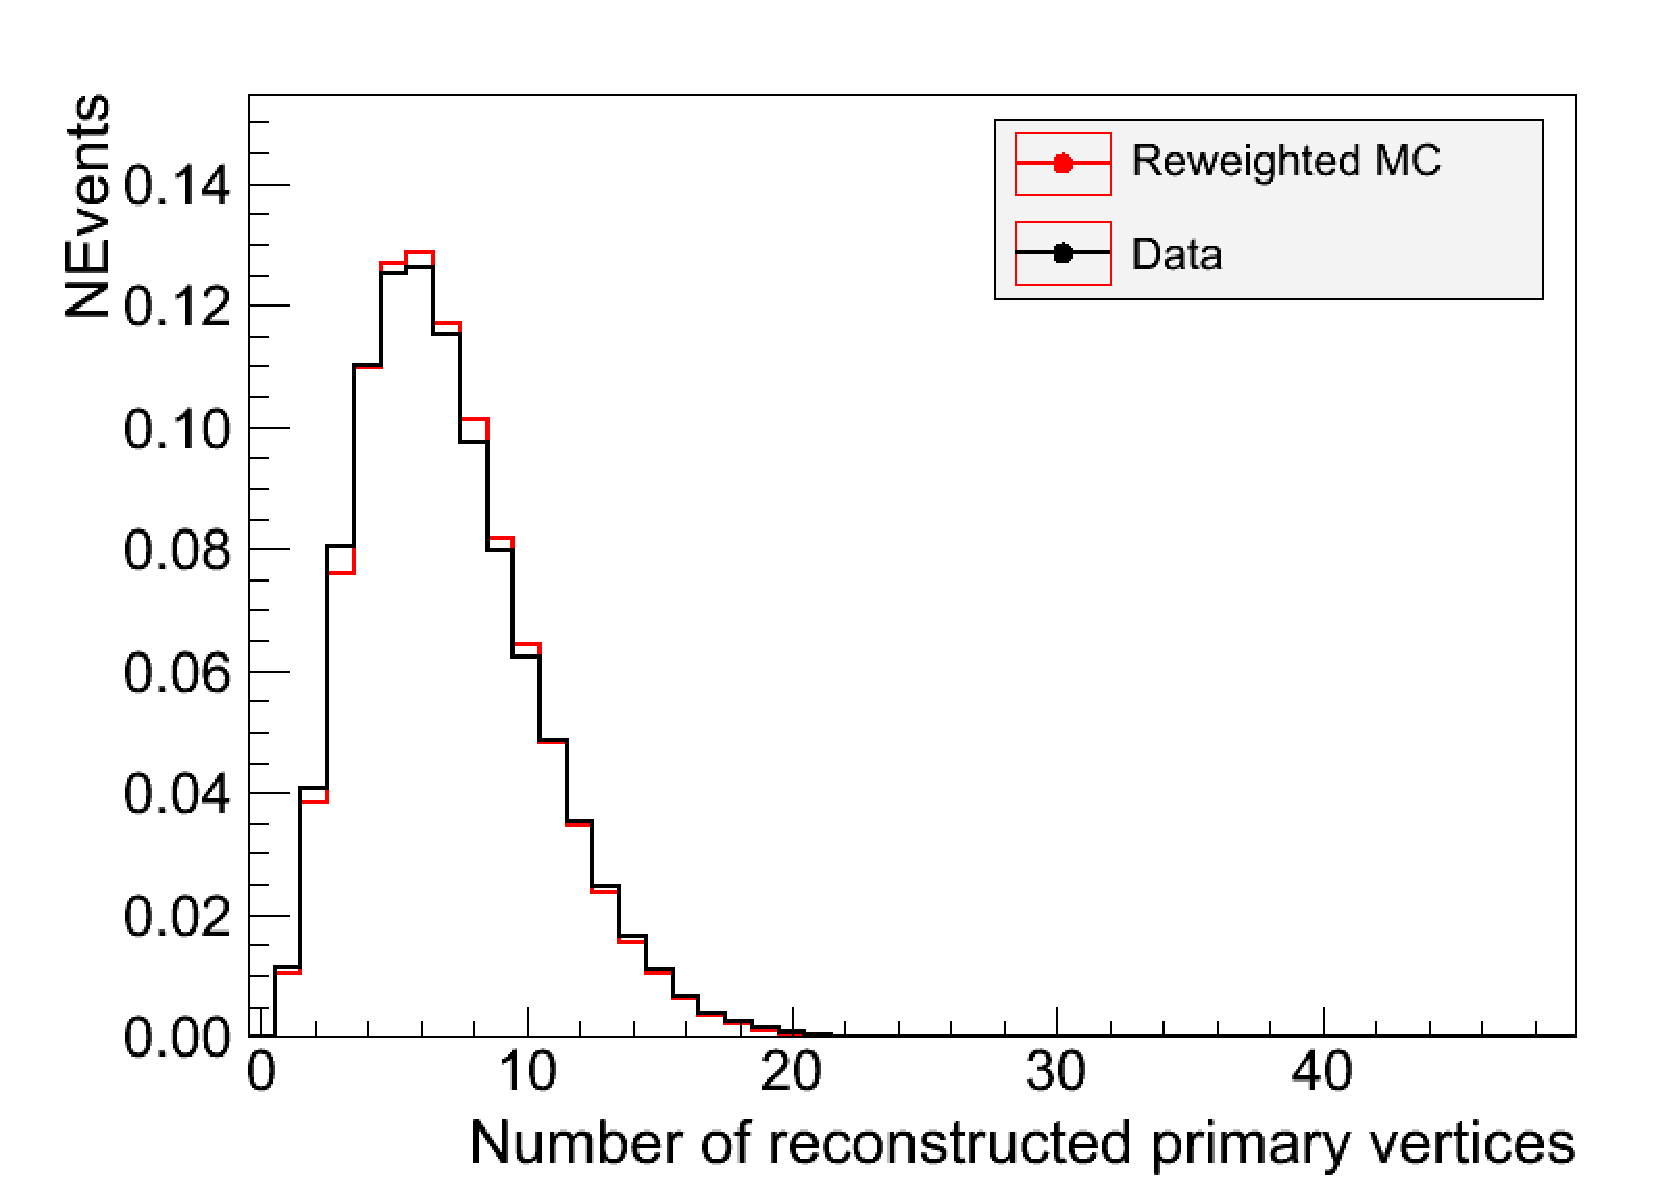
\includegraphics[width=0.45\linewidth]{figures/PileupReweightingValidation_NVtx_SmurfV6DYmm_Full2011.pdf}}
%\subfigure[Event energy density ($\rho$)]{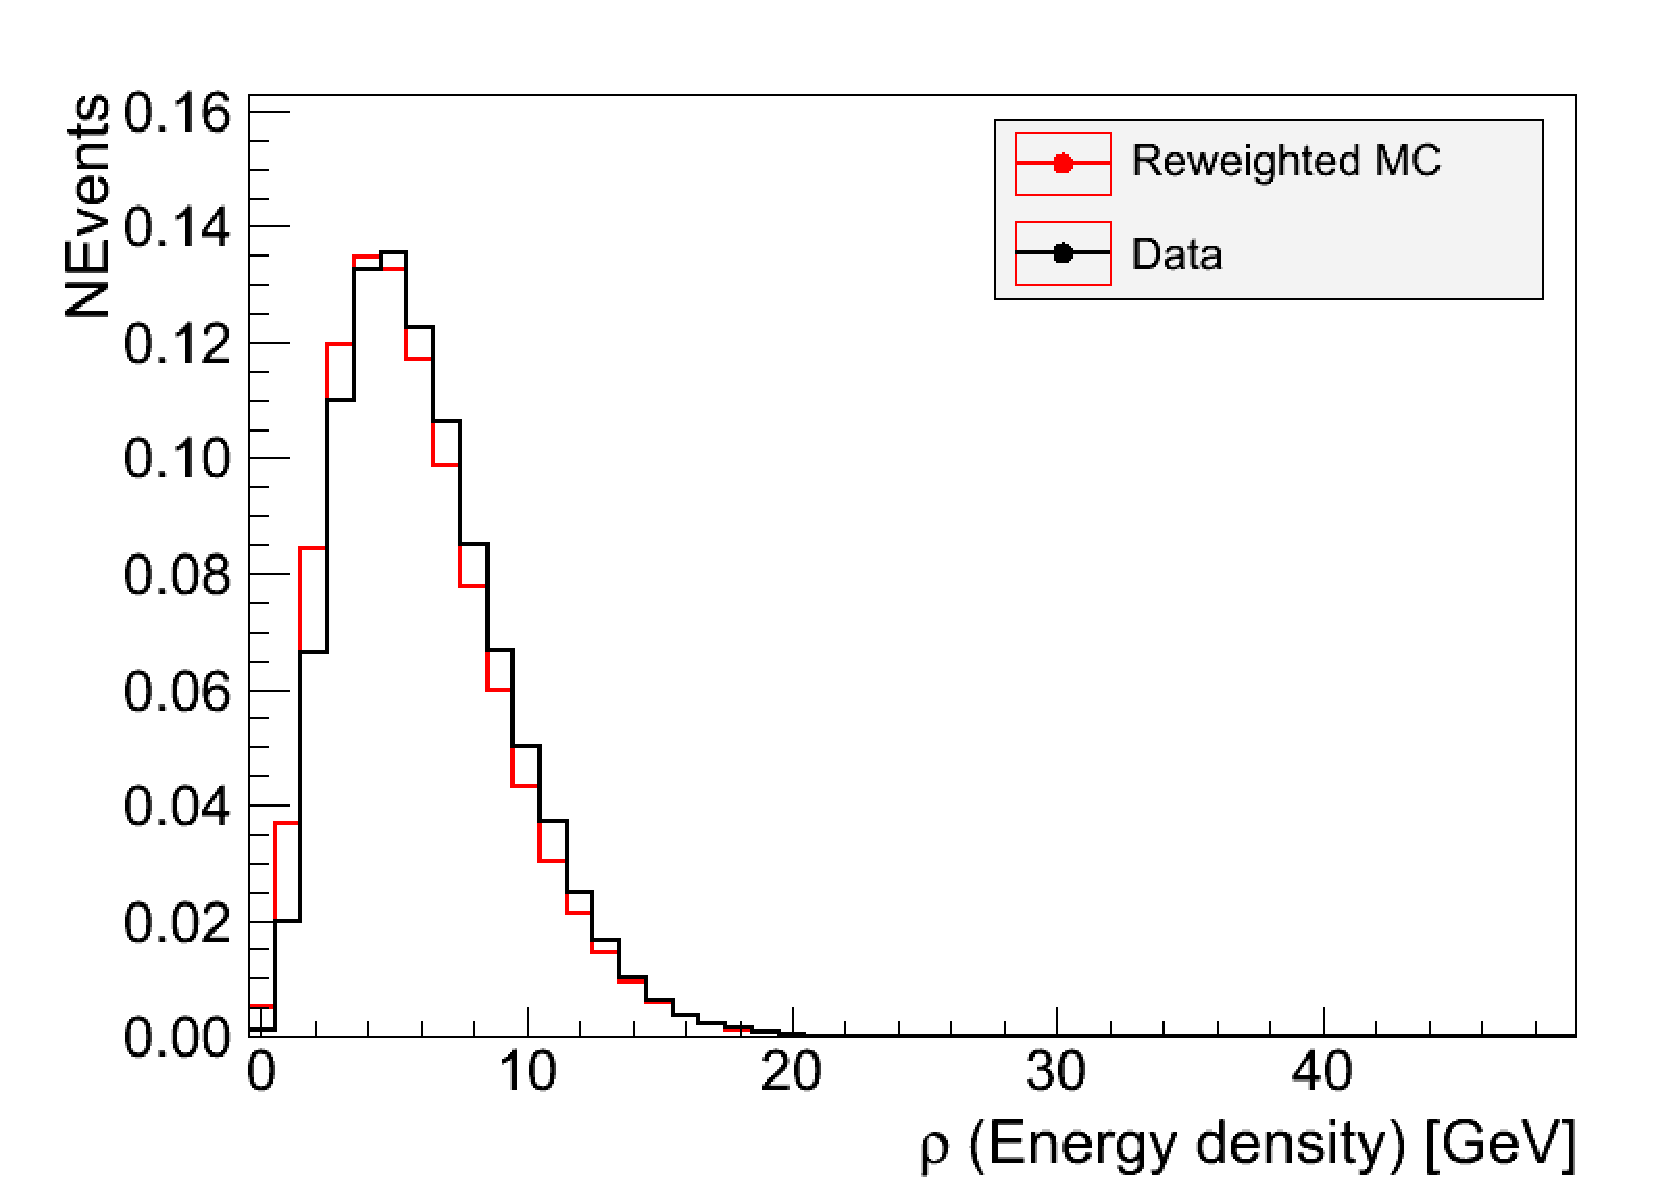
\includegraphics[width=0.45\linewidth]{figures/PileupReweightingValidation_Rho_SmurfV6DYmm_Full2011.pdf}}
\caption{\label{fig:PUValidation_Full2011} Number of reconstructed primary vertices (a) and
the event energy density (b) for data and Monte Carlo reweighted in the number 
of pileup events for the full 2011 dataset.}
\end{center}
\end{figure}

